% !Mode:: "TeX:UTF-8"
\chapter{实践:设计前端}
\begin{mdframed}  
	\textbf{主要目标}
	\begin{enumerate}[labelindent=0em,leftmargin=1.5em]
		\item 实际设计一个视觉里程计前端。
		\item 理解SLAM软件框架是如何搭建的。
		\item 理解在前端设计中容易出现的问题,以及修补的方式。
	\end{enumerate}
\end{mdframed}

本讲是全书比较少见的完全由实践部分组成的一讲。我们将使用前两讲学到的知识,实际书写一个视觉里程计程序。你会管理局部的机器人轨迹与路标点,并体验一下一个软件框架是如何组成的。在操作过程中,我们会遇到许多问题:相机运动过快、图像模糊、误匹配……都会使算法失效。要让程序稳定运行,我们需要处理以上的种种情况,这将带来许多工程实现方面的、有益的讨论。

\newpage 
\section{搭建VO框架}
知晓砖头和水泥的原理,并不代表能够建造伟大的宫殿。

在笔者深爱的《我的世界》游戏中,玩家拥有的只是一些色彩、纹理不同的方块。其性质极其简单,而玩家所要做的只是把这些方块放在空地上而已。理解一个方块至为简单,但实际拿起它们时,初学者往往只能搭建简单的火柴盒房屋,而有经验、有创造力的玩家则可用这些简单的方块建造民居、园林、楼台亭榭,乃至城市(\autoref{fig:mcarchitecture}~)\footnote{左下是笔者的练习作品。右下来自Epicwork团队作品:《圆明园》。}。

\begin{figure}[!htp]
	\centering    
	\includegraphics[width=0.9\linewidth]{designVO/mcarchitecture}\\
	\caption{从简单的事物出发,逐渐搭建越来越复杂但越来越优秀的作品。}
	\label{fig:mcarchitecture}
\end{figure}

在SLAM中,我们认为工程实现和理解算法原理应该至少是同等重要的,甚至更应强调如何书写实际可用的程序。算法的原理,就像一个个方块一样,我们可以清楚明确地讨论它们的原理和性质,但仅仅理解了一个个方块并不能使你建造真正的建筑:它们需要大量的尝试、时间和经验,我们鼓励读者朝更为实际的方向努力——当然这往往是十分复杂的。就像在《我的世界》里那样,你需要掌握各种立柱、墙面、屋顶的结构,墙面的雕花,几何形体角度的计算,这些远远不像讨论每个方块的性质那样简单。

SLAM的具体实现亦是如此,一个实用的程序会有很多的工程设计和技巧(Trick),还需要讨论每一步出现问题之后该如何处理。原则上讲,每个人实现的SLAM都会有所不同,多数时候我们并不能说哪种实现方式就一定是最好的。但是,我们通常会遇到一些共同的问题:“怎么管理地图点”“如何处理误匹配”“如何选择关键帧”,等等。我们希望读者能对这些可能出现的问题产生一些直观的感觉——我们认为这种感觉是非常重要的。

\clearpage
所以,出于对实践的重视,本章我们将带领读者领略一下搭建SLAM框架的过程。就像建筑那样,我们要讨论柱间距、门面宽高比等琐碎但重要的问题。SLAM工程是复杂的。即使我们只保留核心的部分,也会占用大量的篇幅,使本书变得过于繁冗。不过,请注意,尽管完成之后的工程是复杂的,但是中间的“由简到繁”的过程,是值得详细讨论、有学习价值的。所以,我们要从简单的数据结构出发,先来做一个简单的视觉里程计,再慢慢地把一些额外的功能加进来。换言之,我们要把\textbf{从简单到复杂}的过程展现给读者看,这样你才会明白一个库是如何像雪人那样慢慢堆起来的。

本讲的代码放在slambook/project中。由于随着开发过程不断前进,我们会对工程做一些删改,因此它的内容也会发生变化。所以我们会把中间的代码也保留在目录中,以版本号命名,以便读者随时查看、模仿。

\subsection{确定程序框架}
根据前两讲的内容,我们知道视觉里程计分单目、双目、RGB-D三大类。单目视觉相对复杂,而RGB-D最为简单,没有初始化,也没有尺度问题。本着由简入繁的指导思想,我们先从RGB-D做起。为了方便读者做实验,我们将使用数据集而非实际的RGB-D相机(因为不能保证读者人手一台RGB-D相机)。

首先,我们来了解一下Linux程序的组织方式。在编写一个小规模的库时,我们通常会建立一些文件夹,把源代码、头文件、文档、测试数据、配置文件、日志等分类存放,这样会显得很有条理。如果一个库内容很多,我们还会把代码分解成各个独立的小模块,以便测试。读者可以参照OpenCV或g2o的组织方式,看看一个大中型库是如何组织的。例如,OpenCV有core、imgproc、features2d等模块,每个模块分别负责不同的任务。g2o则有core、solvers、types等若干模块。不过在小型程序里,我们也可以把所有的东西糅在一起,称为SLAM库。

现在我们要写的SLAM库是一个小型库,目标是帮读者将本书用到的各种算法融会贯通,书写自己的SLAM程序。挑选一个工程目录,在其下面建立如下文件夹来组织代码文件:

\begin{enumerate}
	\item bin	用来存放可执行的二进制文件。
	\item include/myslam	存放SLAM模块的头文件,主要是.h文件。这种做法的理由是,当把包含目录设到include,引用自己的头文件时,需要写include \texttt{"}myslam/xxx.h\texttt{"},这样不容易和别的库混淆。
	\item src	存放源代码文件,主要是.cpp文件。
	\item test	存放测试用的文件,也是.cpp文件。
	\item lib	存放编译好的库文件。
	\item config	存放配置文件。
	\item cmake\_modules	第三方库的cmake文件,在使用g2o之类的库时会用到它。
\end{enumerate}

以上就是我们的目录结构,如\autoref{fig:proj}~所示。相比于之前每一讲内零零散散地放着的main.cpp,这种做法显得更有条理。接下来,我们会在这些目录里不断地添加新文件,逐渐形成一个完整的程序。

\begin{figure}[!htp]
	\centering
	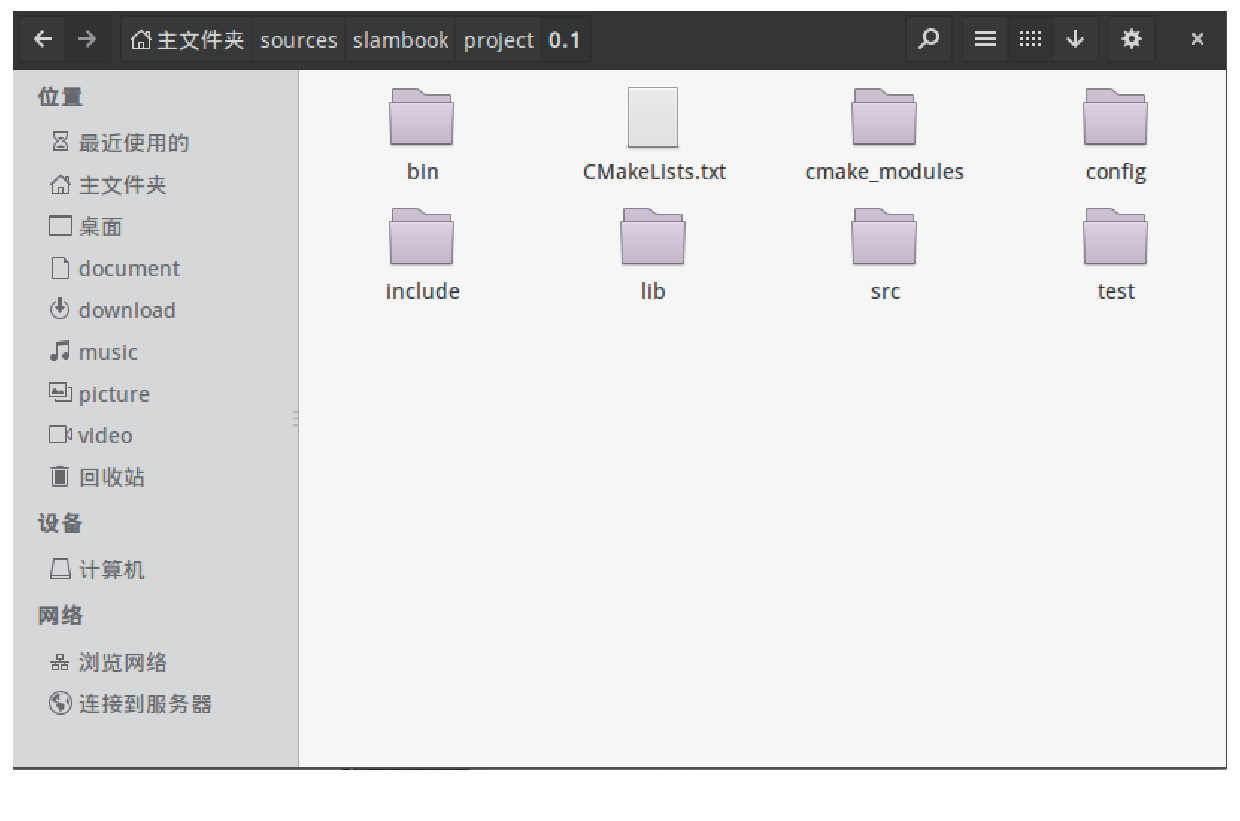
\includegraphics[width=.9\linewidth]{designVO/proj.pdf}
	\caption{工程项目的目录。}
	\label{fig:proj}
\end{figure}

\subsection{确定基本数据结构}
为了让程序跑起来,我们要设计好数据单元,以及程序处理的流程。这好比构成房屋的一个个的柱子和砖块。那么,在一个SLAM程序中,有哪些结构是最基本的呢?我们抽象出以下基本概念:

\begin{enumerate}
	\item \textbf{帧}:帧是相机采集到的图像单位。它主要包含一个图像(RGB-D情形下是一对图像)。此外,还有特征点、位姿、内参等信息。
	
	在视觉SLAM中我们会谈论关键帧(Key-frame)。由于相机采集的数据很多,存储所有的数据显然是不现实的。否则,如果相机放在桌上不动,程序的内存占用也会越来越高直至无法接受。通常的做法是把某些我们认为更重要的帧保存起来,并认为相机轨迹可以用这些关键帧来描述。关键帧如何选择是一个很大的问题,而且基于工程经验,很少有理论上的指导。在本书中我们会使用一个关键帧选择方法,但读者亦可考虑自己提出新的方式。
	
	\item \textbf{路标}:路标点即图像中的特征点。在相机运动后,我们还能估计它们的3D位置。通常,会把路标点放在一个\textbf{地图}当中,并将新来的帧与地图中的路标点进行匹配,估计相机位姿。
\end{enumerate}

\clearpage
帧的位姿与路标的位置估计相当于一个局部的SLAM问题。除此之外,我们还需要一些工具,让程序写起来更流畅。例如:

\begin{enumerate}
	\item \textbf{配置文件}:在写程序过程中你会经常遇到各种各样的参数,比如,相机的内参、特征点的数量、匹配时选择的比例,等等。你可以把这些数写在程序中,但那不是一个好习惯。你会经常修改这些参数,但每次修改后都要重新编译一遍程序。当其数量越来越多时,修改就变得越来越困难。所以,更好的方式是在外部定义一个配置文件,程序运行时读取该配置文件中的参数值。这样,每次只要修改配置文件内容就行了,不必对程序本身做任何修改。
	\item \textbf{坐标变换}:你会经常需要在坐标系间进行坐标变换,例如,世界坐标到相机坐标、相机坐标到归一化相机坐标、归一化相机坐标到像素坐标,等等。定义一个类把这些操作都放在一起将更方便。
\end{enumerate}

下面我们就来定义帧、路标这几个概念,在C++中都以类来表示。我们尽量保证一个类有单独的头文件和源文件,避免把许多个类放在同一个文件中。然后,把函数声明放在头文件,实现放在源文件中(除非函数很短,也可以写在头文件中)。我们参照Google的命名规范,同时考虑尽量以初学者也能看懂的方式来写程序。由于我们的程序是偏向算法而非软件工程的,所以不讨论复杂的类继承关系、接口、模板等,而更关注\textbf{算法的正确实现,以及是否便于扩展}。我们会把数据成员设置为公有,尽管这在C++软件设计中是应该避免的,如果读者愿意,也可以把它们改成private或protected接口,并添加设置和获取接口。在过程较为复杂的算法中,我们会把它分解成若干步骤,例如特征提取和匹配应该分别在不同的函数中实现,这样,当我们想修改算法流程时,就不需要修改整个运行流程,只需调整局部的处理方式即可。

现在,让我们开始写VO。我们把这个版本定为0.1版,表示这是刚开始的阶段。我们一共写5个类:Frame为帧,Camera为相机模型,MapPoint为特征点/路标点,Map管理特征点,Config提供配置参数。它们的关系如\autoref{fig:class0.1}~所示。我们现在只写它们的数据成员和常用方法,而在后面用到更多内容时再行添加。

\begin{figure}[!ht]
	\centering
	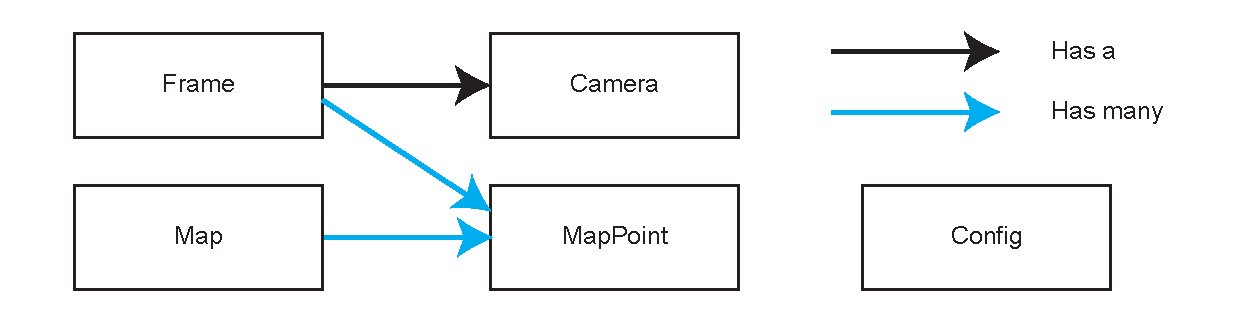
\includegraphics[width=1.0\linewidth]{designVO/class.pdf}
	\caption{基本类的关系示意图。}
	\label{fig:class0.1}
\end{figure}

Camera类最简单,我们先来实现它。
\clearpage

\subsection{Camera类}
Camera类存储相机的内参和外参,并完成相机坐标系、像素坐标系和世界坐标系之间的坐标变换。当然,在世界坐标系中你需要一个相机的(变动的)外参,我们以参数的形式传入。

\begin{lstlisting}[language=c++,caption=slambook/project/0.1/include/myslam/camera.h]
#ifndef CAMERA_H
#define CAMERA_H
#include "myslam/common_include.h"
namespace myslam
{
// Pinhole RGB-D camera model
class Camera
{
public:
	typedef std::shared_ptr<Camera> Ptr;
	float   fx_, fy_, cx_, cy_, depth_scale_;  // Camera intrinsics 
	
	Camera();
	Camera ( float fx, float fy, float cx, float cy, float depth_scale=0 ) :
	fx_ ( fx ), fy_ ( fy ), cx_ ( cx ), cy_ ( cy ), depth_scale_ ( depth_scale )
	{}
	
	// coordinate transform: world, camera, pixel
	Vector3d world2camera( const Vector3d& p_w, const SE3& T_c_w );
	Vector3d camera2world( const Vector3d& p_c, const SE3& T_c_w );
	Vector2d camera2pixel( const Vector3d& p_c );
	Vector3d pixel2camera( const Vector2d& p_p, double depth=1 ); 
	Vector3d pixel2world ( const Vector2d& p_p, const SE3& T_c_w, double depth=1 );
	Vector2d world2pixel ( const Vector3d& p_w, const SE3& T_c_w );
};
}
#endif // CAMERA_H
\end{lstlisting}

说明如下(由上往下):
\begin{enumerate}
	\item 在这个简单的例子中,我们给出了防止头文件重复引用的ifndef宏定义。如果没有这个宏,在两处引用此头文件时将出现类的重复定义。所以,在每个程序头文件里都会定义这样一个宏。
	\item 我们用命名空间namespace myslam将类定义包裹起来(因为是我们自己写的SLAM,所以命名空间就叫myslam了)。命名空间可以防止我们不小心定义出别的库里同名的函数,也是一种比较安全和规范的做法。由于宏定义和命名空间在每个文件中都会写一遍,所以我们只在这里稍加介绍,后面将略去。
	\item 我们把一些常用的头文件放在common\_include.h文件中,这样就可以避免每次书写很长的一串include。
	\item 我们把智能指针定义成Camera的指针类型,因此以后在传递参数时使用Camera::Ptr类型即可。
	\item 我们用Sophus::SE3来表达相机的位姿。Sophus库在李代数一讲介绍过。
\end{enumerate}

在源文件中,给出Camera方法的实现:
\begin{lstlisting}[language=c++,caption=slambook/project/0.1/src/camera.cpp]
#include "myslam/camera.h"
namespace myslam
{

Camera::Camera()
{
}

Vector3d Camera::world2camera ( const Vector3d& p_w, const SE3& T_c_w )
{
	return T_c_w*p_w;
}

Vector3d Camera::camera2world ( const Vector3d& p_c, const SE3& T_c_w )
{
	return T_c_w.inverse() *p_c;
}

Vector2d Camera::camera2pixel ( const Vector3d& p_c )
{
	return Vector2d (
		fx_ * p_c ( 0,0 ) / p_c ( 2,0 ) + cx_,
		fy_ * p_c ( 1,0 ) / p_c ( 2,0 ) + cy_
	);
}

Vector3d Camera::pixel2camera ( const Vector2d& p_p, double depth )
{
	return Vector3d (
		( p_p ( 0,0 )-cx_ ) *depth/fx_,
		( p_p ( 1,0 )-cy_ ) *depth/fy_,
		depth
	);
}

Vector2d Camera::world2pixel ( const Vector3d& p_w, const SE3& T_c_w )
{
	return camera2pixel ( world2camera ( p_w, T_c_w ) );
}

Vector3d Camera::pixel2world ( const Vector2d& p_p, const SE3& T_c_w, double depth )
{
	return camera2world ( pixel2camera ( p_p, depth ), T_c_w );
}
}
\end{lstlisting}

读者可以对照一下这些方法是否和第5讲的内容一致。它们完成了像素坐标系、相机坐标系和世界坐标系间的坐标变换。

\subsection{Frame类}
下面来考虑Frame类。Frame类是基本数据单元,在许多地方会用到,但现在是初期设计阶段,我们还不清楚以后可能新加的内容。所以这里的Frame类只提供基本的数据存储和接口。如果之后有新增的内容,再继续往里添加。

\begin{lstlisting}[language=c++,caption=slambook/project/0.1/include/myslam/frame.h]
class Frame
{
public:
	typedef std::shared_ptr<Frame> Ptr;
	unsigned long  id_; // id of this frame
	double time_stamp_; // when it is recorded
	SE3 T_c_w_; // transform from world to camera
	Camera::Ptr camera_; // Pinhole RGB-D Camera model 
	Mat color_, depth_; // color and depth image 

public: // data members 
	Frame();
	Frame( long id, double time_stamp=0, SE3 T_c_w=SE3(), Camera::Ptr camera=nullptr, Mat color=Mat(), Mat depth=Mat() );
	~Frame();

	// factory function
	static Frame::Ptr createFrame(); 
	
	// find the depth in depth map
	double findDepth( const cv::KeyPoint& kp );
	
	// Get Camera Center
	Vector3d getCamCenter() const;
	
	// check if a point is in this frame 
	bool isInFrame( const Vector3d& pt_world );
};
\end{lstlisting}

在Frame中,我们定义了ID、时间戳、位姿、相机、图像这几个量,这应该是一个帧当中含有的最重要的信息。在方法中,我们提取了几个重要的方法:创建Frame、寻找给定点对应的深度、获取相机光心、判断某个点是否在视野内,等等。它们的实现是比较平凡的,请读者参考frame.cpp了解这些函数的具体实现。

\subsection{MapPoint类}
MapPoint表示路标点。我们将估计它的世界坐标,并且会拿当前帧提取到的特征点与地图中的路标点匹配,来估计相机的运动,因此还需要存储它对应的描述子。此外,我们会记录一个点被观测到的次数和被匹配的次数,作为评价其好坏程度的指标。

\begin{lstlisting}[language=c++,caption=slambook/project/0.1/include/myslam/mappoint.h]
class MapPoint
{
public:
	typedef shared_ptr<MapPoint> Ptr;
	unsigned long      id_; // ID
	Vector3d    pos_;       // Position in world
	Vector3d    norm_;      // Normal of viewing direction 
	Mat         descriptor_; // Descriptor for matching 
	int         observed_times_;    // being observed by feature matching algo.
	int         correct_times_;     // being an inliner in pose estimation

	MapPoint();
	MapPoint( long id, Vector3d position, Vector3d norm );

	// factory function
	static MapPoint::Ptr createMapPoint();
};
\end{lstlisting}

同样,读者可以浏览src/map.cpp查看其实现。目前为止我们只考虑这些数据成员的初始化问题。

\subsection{Map类}
Map类管理着所有的路标点,并负责添加新路标、删除不好的路标等工作。VO的匹配过程只要和Map打交道即可。当然Map也会有很多操作,但现阶段我们只定义主要的数据结构。

\begin{lstlisting}[language=c++,caption=slambook/project/0.1/include/myslam/map.h]
class Map
{
public:
	typedef shared_ptr<Map> Ptr;
	unordered_map<unsigned long, MapPoint::Ptr >  map_points_;        // all landmarks
	unordered_map<unsigned long, Frame::Ptr >     keyframes_;         // all key-frames

	Map() {}
	
	void insertKeyFrame( Frame::Ptr frame );
	void insertMapPoint( MapPoint::Ptr map_point );
};
\end{lstlisting}

Map类中实际存储了各个关键帧和路标点,既需要随机访问,又需要随时插入和删除,因此我们使用散列(Hash)来进行存储。

\subsection{Config类}

Config类负责参数文件的读取,并在程序的任意地方都可随时提供参数的值。所以我们把Config写成单件模式(Singleton)。它只有一个全局对象,当我们设置参数文件时,创建该对象并读取参数文件,随后就可以在任意地方访问参数值,最后在程序结束时自动销毁。

\begin{lstlisting}[language=c++,caption=slambook/project/0.1/include/myslam/config.h]
class Config
{
private:
	static std::shared_ptr<Config> config_; 
	cv::FileStorage file_;
	
	Config () {} // private constructor makes a singleton
public:
	~Config();  // close the file when deconstructing 
	
	// set a new config file 
	static void setParameterFile( const std::string& filename ); 
	
	// access the parameter values
	template< typename T >
	static T get( const std::string& key )
	{
		return T( Config::config_->file_[key] );
	}
};
\end{lstlisting}

说明如下:
\begin{enumerate}
	\item 我们把构造函数声明为私有,防止这个类的对象在别处建立,它只能在setParameterFile时构造。实际构造的对象是Config的智能指针:static shared\_ptr\\<Config> config_。用智能指针的原因是可以自动析构,省得我们再调一个别的函数来做析构。
	\item 在文件读取方面,我们使用OpenCV提供的FileStorage类。它可以读取一个YAML文件,且可以访问其中任意一个字段。由于参数实质值可能为整数、浮点数或字符串,所以我们通过一个模板函数get来获得任意类型的参数值。
\end{enumerate}

下面是Config的实现。注意,我们把单例模式的全局指针定义在此源文件中了:
\begin{lstlisting}[language=c++,caption=slambook/project/0.1/src/config.cpp]
void Config::setParameterFile( const std::string& filename )
{
	if ( config_ == nullptr )
		config_ = shared_ptr<Config>(new Config);
	config_->file_ = cv::FileStorage( filename.c_str(), cv::FileStorage::READ );
	if ( config_->file_.isOpened() == false )
	{
		std::cerr<<"parameter file "<<filename<<" does not exist."<<std::endl;
		config_->file_.release();
		return ;
	}
}
Config::~Config()
{
	if ( file_.isOpened() )
		file_.release();
}
shared_ptr<Config> Config::config_ = nullptr;
\end{lstlisting}

在实现中,我们只要判断一下参数文件是否存在即可。定义了这个Config类后,我们可以在任何地方获取参数文件里的参数。例如,当想要定义相机的焦距$f_x$时,按照如下步骤操作即可:

\begin{enumerate}
	\item 在参数文件中加入:“Camera.fx: 500”。
	\item 在代码中使用:
\begin{lstlisting}[language=c++]
myslam::Config::setParameterFile("parameter.yaml");
double fx = myslam::Config::get<double> ("Camera.fx");
\end{lstlisting}
	就能获得$f_x$的值了。
\end{enumerate}
当然,参数文件的实现方法绝对不止这一种。我们主要从程序开发上的便利角度来考虑这个实现,读者当然也可以用更简单的方式来实现参数的配置。

至此,我们定义了SLAM程序的基本数据结构,书写了若干个基本类。这好比是造房子的砖头和水泥。你可以调用cmake编译这个0.1版,尽管它还没有实质性的功能。接下来我们来考虑把前面讲过的VO算法加到工程中,并做一些测试来调整各算法的性能。注意,笔者会刻意地暴露某些设计的问题,所以你看到的实现不见得就是最好的(或者足够好的)。

\section{基本的VO:特征提取和匹配}
下面我们来实现VO,先来考虑特征点法。它的任务是,根据输入的图像,计算相机运动和特征点位置。前面我们讨论的都是在两两帧间的位姿估计,然而我们将发现,仅凭两帧的估计是不够的。我们会把特征点缓存成一个小地图,计算当前帧与地图之间的位置关系。但那样程序会复杂一些,所以,让我们先订个小目标,暂时从两两帧间的运动估计出发。

\subsection{两两帧的视觉里程计}
如果像前面两讲一样,只关心两个帧之间的运动估计,并且不优化特征点的位置。然后把估得的位姿“串”起来,也能得到一条运动轨迹。这种方式可以看成两两帧间的(Pairwise)无结构(Structureless)的VO,实现起来最为简单,但是效果不佳。为什么不佳呢?我们一起来体验一下。记该工程为0.2版本。

两两帧之间的VO工作示意图如\autoref{fig:pairwise-VO}~所示。在这种VO里,我们定义了参考帧(Reference)和当前帧(Current)这两个概念。以参考帧为坐标系,我们把当前帧与它进行特征匹配,并估计运动关系。假设参考帧相对世界坐标的变换矩阵为$\bm{T}_\mathrm{rw}$,当前帧与世界坐标系间为$\bm{T}_\mathrm{cw}$,则待估计的运动与这两个帧的变换矩阵构成左乘关系:
\[
\bm{T}_\mathrm{cr}, \quad \mathrm{s.t.} \quad \bm{T}_\mathrm{cw} = \bm{T}_\mathrm{cr} \bm{T}_\mathrm{rw}.
\]

在$t-1$到$t$时刻,我们以$t-1$为参考,求取$t$时刻的运动。这可以通过特征点匹配、光流或直接法得到,但这里我们\textbf{只关心运动,不关心结构}。换句话说,只要通过特征点成功求出了运动,我们就不再需要这一帧的特征点了。这种做法当然会有缺陷,但是忽略掉数量庞大的特征点可以节省许多的计算量。然后,在$t$到$t+1$时刻,我们又以$t$时刻为参考帧,考虑$t$到$t+1$间的运动关系。如此往复,就得到了一条运动轨迹。

\begin{figure}[!ht]
	\centering    
	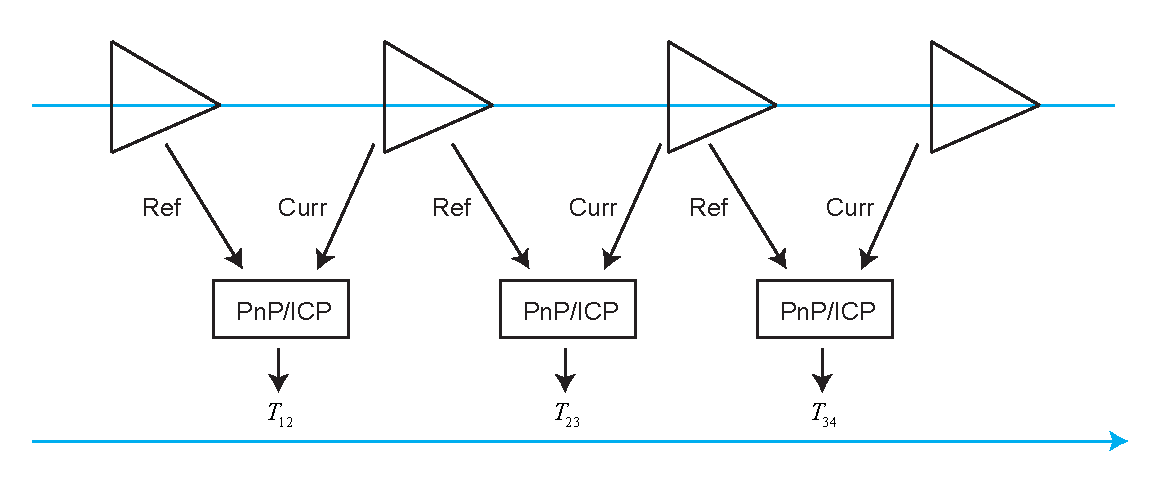
\includegraphics[width=0.85\linewidth]{designVO/pairwiseVO}\\
	\caption{两两帧的VO示意图。}
	\label{fig:pairwise-VO}
\end{figure}

这种VO的工作方式是简单的,不过实现也可以有若干种。我们以传统的匹配特征点——求PnP的方法为例实现一遍。希望读者能够结合之前几讲的知识,自己实现一下光流/直接法或ICP求运动的VO。在匹配特征点的方式中,最重要的是参考帧与当前帧之间的特征匹配关系,它的流程可归纳如下:

\begin{mdframed}
\begin{enumerate}
	\item 对新来的当前帧,提取关键点和描述子。
	\item 如果系统未初始化,以该帧为参考帧,根据深度图计算关键点的3D位置,返回第1步。
	\item 估计参考帧与当前帧间的运动。
	\item 判断上述估计是否成功。
	\item 若成功,把当前帧作为新的参考帧,返回第1步。
	\item 若失败,计录连续丢失帧数。当连续丢失超过一定帧数时,置VO状态为丢失,算法结束。若未超过,返回第1步。
\end{enumerate}
\end{mdframed}

VisualOdometry类给出了上述算法的实现。

\begin{lstlisting}[language=c++,caption=slambook/project/0.2/include/myslam/visual\_odometry.h]
class VisualOdometry
{
public:
	typedef shared_ptr<VisualOdometry> Ptr;
	enum VOState {
		INITIALIZING=-1,
		OK=0,
		LOST
	};

	VOState     state_; // current VO status
	Map::Ptr    map_; // map with all frames and map points
	Frame::Ptr  ref_; // reference frame 
	Frame::Ptr  curr_; // current frame 

	cv::Ptr<cv::ORB> orb_; // orb detector and computer 
	vector<cv::Point3f> pts_3d_ref_; // 3d points in reference frame 
	vector<cv::KeyPoint> keypoints_curr_; // keypoints in current frame
	Mat descriptors_curr_; // descriptor in current frame 
	Mat descriptors_ref_; // descriptor in reference frame 
	vector<cv::DMatch> feature_matches_;

	SE3 T_c_r_estimated_; // the estimated pose of current frame 
	int num_inliers_; // number of inlier features in icp
	int num_lost_; // number of lost times

	// parameters 
	int num_of_features_; // number of features
	double scale_factor_; // scale in image pyramid
	int level_pyramid_; // number of pyramid levels
	float match_ratio_; // ratio for selecting  good matches
	int max_num_lost_; // max number of continuous lost times
	int min_inliers_; // minimum inliers
	
	double key_frame_min_rot; // minimal rotation of two key-frames
	double key_frame_min_trans; // minimal translation of two key-frames

public: // functions 
	VisualOdometry();
	~VisualOdometry();

	bool addFrame( Frame::Ptr frame );      // add a new frame 

protected:  
	// inner operation 
	void extractKeyPoints();
	void computeDescriptors(); 
	void featureMatching();
	void poseEstimationPnP(); 
	void setRef3DPoints();
	
	void addKeyFrame();
	bool checkEstimatedPose(); 
	bool checkKeyFrame();
};
\end{lstlisting}

关于这个VisualOdometry类,有几点需要解释:

\begin{enumerate}
	\item VO本身有若干种状态:设定第一帧、顺利跟踪或丢失,你可以把它看成一个有限状态机(Finite State Machine,FSM)。当然状态也可以有更多种,例如,单目VO至少还有一个初始化状态。在我们的实现中,考虑最简单的三个状态:初始化、正常、丢失。
	\item 我们把一些中间变量定义在类中,这样可省去复杂的参数传递。因为它们都是定义在类内部的,所以各个函数都可以访问它们。
	\item 特征提取和匹配当中的参数从参数文件中读取。例如:
\begin{lstlisting}[language=c++]
VisualOdometry::VisualOdometry() :
	state_ ( INITIALIZING ), ref_ ( nullptr ), curr_ ( nullptr ), map_ ( new Map ), num_lost_ ( 0 ), num_inliers_ ( 0 )
{
	num_of_features_    = Config::get<int> ( "number_of_features" );
	scale_factor_       = Config::get<double> ( "scale_factor" );
	level_pyramid_      = Config::get<int> ( "level_pyramid" );
	match_ratio_        = Config::get<float> ( "match_ratio" );
	...
}
	\end{lstlisting} 
	\item addFrame函数是外部调用的接口。使用VO时,将图像数据装入Frame类后,调用addFrame估计其位姿。该函数根据VO所处的状态实现不同的操作:
\begin{lstlisting}[language=c++]
bool VisualOdometry::addFrame ( Frame::Ptr frame )
{
	switch ( state_ )
	{
	case INITIALIZING:
	{
		state_ = OK;
		curr_ = ref_ = frame;
		map_->insertKeyFrame ( frame );
		// extract features from first frame 
		extractKeyPoints();
		computeDescriptors();
		// compute the 3d position of features in ref frame 
		setRef3DPoints();
		break;
	}
	case OK:
	{
		curr_ = frame;
		extractKeyPoints();
		computeDescriptors();
		featureMatching();
		poseEstimationPnP();
		if ( checkEstimatedPose() == true ) // a good estimation
		{
			curr_->T_c_w_ = T_c_r_estimated_ * ref_->T_c_w_;  // T_c_w = T_c_r*T_r_w 
			ref_ = curr_;
			setRef3DPoints();
			num_lost_ = 0;
			if ( checkKeyFrame() == true ) // is a key-frame
			{
				addKeyFrame();
			}
		}
		else // bad estimation due to various reasons
		{
			num_lost_++;
			if ( num_lost_ > max_num_lost_ )
			{
				state_ = LOST;
			}
			return false;
		}
		break;
	}
	case LOST:
	{
		cout<<"vo has lost."<<endl;
		break;
	}
	}
	return true;
}
\end{lstlisting}
\end{enumerate}

值得一提的是,由于各种原因,我们设计的上述VO算法,每一步都有可能失败。例如,图片中不易提特征、特征点缺少深度值、误匹配、运动估计出错,等等。因此,要设计一个健壮的VO,必须(最好是显式地)考虑到上述所有可能出错的地方——那自然会使程序变得非常复杂。我们在checkEstimatedPose中根据内点(inlier)的数量及运动的大小做一个简单的检测:认为内点不可太少,而运动不可能过大。当然,读者也可以思考其他检测问题的手段,尝试一下效果。

我们略去VisualOdometry类其余的实现,读者可在GitHub上找到所有的源代码。最后,我们在test中加入该VO的测试程序,使用数据集观察估计的运动效果:

\begin{lstlisting}[language=c++,caption=slambook/project/0.2/test/run\_vo.cpp]
int main ( int argc, char** argv )
{
	if ( argc != 2 )
	{
		cout<<"usage: run_vo parameter_file"<<endl;
		return 1;
	}

	myslam::Config::setParameterFile ( argv[1] );
	myslam::VisualOdometry::Ptr vo ( new myslam::VisualOdometry );

	string dataset_dir = myslam::Config::get<string> ( "dataset_dir" );
	cout<<"dataset: "<<dataset_dir<<endl;
	ifstream fin ( dataset_dir+"/associate.txt" );
	if ( !fin )
	{
		cout<<"please generate the associate file called associate.txt!"<<endl;
		return 1;
	}

	vector<string> rgb_files, depth_files;
	vector<double> rgb_times, depth_times;
	while ( !fin.eof() )
	{
		string rgb_time, rgb_file, depth_time, depth_file;
		fin>>rgb_time>>rgb_file>>depth_time>>depth_file;
		rgb_times.push_back ( atof ( rgb_time.c_str() ) );
		depth_times.push_back ( atof ( depth_time.c_str() ) );
		rgb_files.push_back ( dataset_dir+"/"+rgb_file );
		depth_files.push_back ( dataset_dir+"/"+depth_file );
		
		if ( fin.good() == false )
			break;
	}
	
	myslam::Camera::Ptr camera ( new myslam::Camera );
	
	// visualization
	cv::viz::Viz3d vis("Visual Odometry");
	cv::viz::WCoordinateSystem world_coor(1.0), camera_coor(0.5);
	cv::Point3d cam_pos( 0, -1.0, -1.0 ), cam_focal_point(0,0,0), cam_y_dir(0,1,0);
	cv::Affine3d cam_pose = cv::viz::makeCameraPose( cam_pos, cam_focal_point, cam_y_dir );
	vis.setViewerPose( cam_pose );
	
	world_coor.setRenderingProperty(cv::viz::LINE_WIDTH, 2.0);
	camera_coor.setRenderingProperty(cv::viz::LINE_WIDTH, 1.0);
	vis.showWidget( "World", world_coor );
	vis.showWidget( "Camera", camera_coor );
	
	cout<<"read total "<<rgb_files.size() <<" entries"<<endl;
	for ( int i=0; i<rgb_files.size(); i++ )
	{
		Mat color = cv::imread ( rgb_files[i] );
		Mat depth = cv::imread ( depth_files[i], -1 );
		if ( color.data==nullptr || depth.data==nullptr )
		break;
		myslam::Frame::Ptr pFrame = myslam::Frame::createFrame();
		pFrame->camera_ = camera;
		pFrame->color_ = color;
		pFrame->depth_ = depth;
		pFrame->time_stamp_ = rgb_times[i];
		
		boost::timer timer;
		vo->addFrame ( pFrame );
		cout<<"VO costs time: "<<timer.elapsed()<<endl;
		
		if ( vo->state_ == myslam::VisualOdometry::LOST )
			break;
		SE3 Tcw = pFrame->T_c_w_.inverse();
		
		// show the map and the camera pose 
		cv::Affine3d M(
			cv::Affine3d::Mat3( 
				Tcw.rotation_matrix()(0,0), Tcw.rotation_matrix()(0,1), Tcw.rotation_matrix()(0,2),
				Tcw.rotation_matrix()(1,0), Tcw.rotation_matrix()(1,1), Tcw.rotation_matrix()(1,2),
				Tcw.rotation_matrix()(2,0), Tcw.rotation_matrix()(2,1), Tcw.rotation_matrix()(2,2)
			), 
			cv::Affine3d::Vec3(
				Tcw.translation()(0,0), Tcw.translation()(1,0), Tcw.translation()(2,0)
			)
		);
		cv::imshow("image", color );
		cv::waitKey(1);
		vis.setWidgetPose( "Camera", M);
		vis.spinOnce(1, false);
	}
	return 0;
}
\end{lstlisting}

为了运行这个程序,需要做几件事:

\begin{enumerate}
	\item 因为我们用OpenCV 3的viz模块显示估计位姿,请确保你安装的是OpenCV 3,并且viz模块也已编译安装。
	\item 准备TUM数据集中的其中一个。简单起见,笔者推荐fr1\_xyz那一个。请使用associate.py生成一个配对文件associate.txt。关于TUM数据集格式,在~\ref{sec:LKFlow}~节中已介绍。
	\item 在config/default.yaml中填写你的数据集所在路径,参照笔者的写法即可。然后,用
\begin{lstlisting}[language=sh]
bin/run_vo config/default.yaml
\end{lstlisting}
	执行程序,就可以看到实时的演示了,如\autoref{fig:vo02exp}~所示。
\end{enumerate}

\begin{figure}[!htp]
	\centering    
	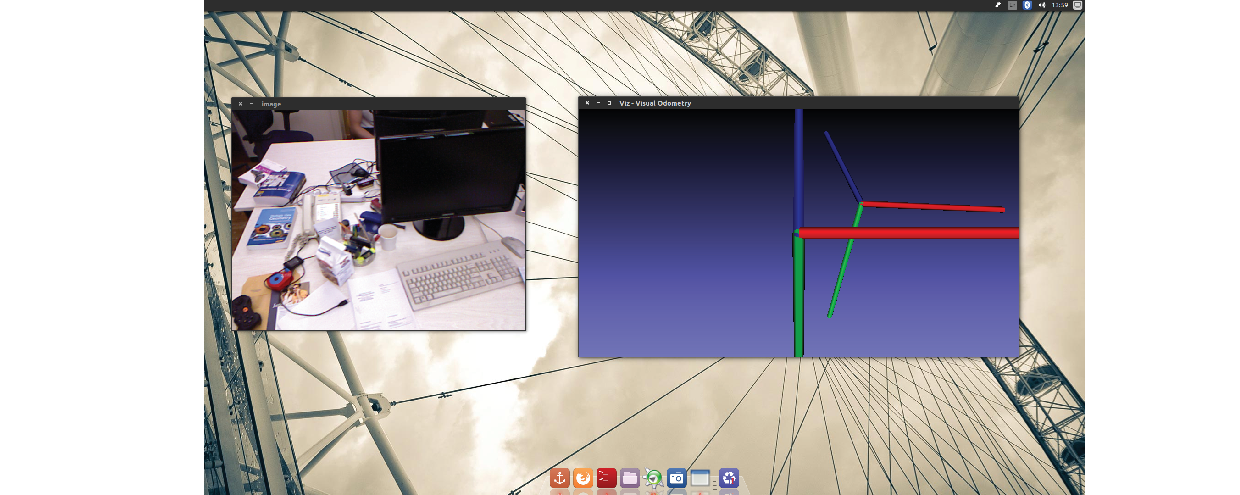
\includegraphics[width=0.9\linewidth]{designVO/vo02exp}\\
	\caption{0.2版本的VO演示。}
	\label{fig:vo02exp}
\end{figure}

在演示程序中,你可以看到当前帧的图像与它的估计位置。我们画出了世界坐标系的坐标轴(大)与当前帧的坐标轴(小),颜色与轴的对应关系为:蓝色—Z,红\mbox{色—X},绿色—Y。你可以直观地感受到相机的运动,它与我们人类的感觉是大致相符的,尽管效果距离预想还有一定的差距。程序还输出了VO单次计算的用时,在笔者的机器上,能够以每次花费30ms左右的速度运行。减少特征点数量可以提高运算速度。读者可以修改运行参数和数据集,看看它在各种情况下的表现。

\subsection{讨论}
本节,我们实现了一个简单的两两帧间的视觉里程计,然而不管从速度还是精度上来说,它的效果都不理想。似乎这种看似简单的思路并不能得到很好的结果。我们来考虑一下有哪些可能的原因:

\begin{enumerate}
	\item
	在位姿估计时,我们使用了RANSAC求出的PnP解。由于RANSAC只采用少数几个随机点来计算PnP,虽然能够确定inlier,但该方法容易受噪声影响。在3D−2D点存在噪声的情形下,我们要用RANSAC的解作为初值,再用非线性优化求一个最优值。下一节将说明这种做法是优于现在的做法的。
	
	\item 
	由于现在的VO是无结构的,特征点的3D位置被当作真值来估计运动。但实际上,RGB-D的深度图必定带有一定的误差,特别是那些深度过近或过远的地方。并且,由于特征点往往位于物体的边缘处,那些地方的深度测量值通常是不准确的。所以现在的做法不够精确,我们需要把特征点也放在一起优化。
	
	\item 只考虑参考帧/当前帧的方式,一方面使得位姿估计过于依赖参考帧。如果参考帧质量太差,比如,出现严重遮挡、光照变化的情况下,跟踪容易丢失。并且,当参考帧位姿估计不准时,还会出现明显的\textbf{漂移}。另一方面,仅使用两帧数据显然没有充分地利用所有的信息。更自然的方式是比较当前帧和地图,而不是比较当前帧和参考帧。于是,我们要关心\textbf{如何把当前帧与地图进行匹配,以及如何优化地图点}的问题。
	
	\item 由于输出了各步骤的运行时间,我们可以对计算量有一个大概的了解(\autoref{table:runtime-exp1})。
	
	\begin{table}[!ht]
		\centering
		\caption{某一次循环的各步骤用时}
		\label{table:runtime-exp1}
			\begin{tabu}{c|c|c|c|c|c|c}
				\toprule
				项目 & 特征提取 & 描述子计算 & 特征匹配 & PnP求解 & 其他 & 总计 \\ \midrule
				时间 & 0.0102 & 0.0087 & 0.0118 & 0.0011 & 0.0001 & 0.0319 \\ 
				\bottomrule
			\end{tabu} 
	\end{table}
	
	可以看到,特征点的提取和匹配占用了绝大多数的计算时间,而看似复杂的PnP优化,计算量与之相比基本可以忽略。因此,如何提高特征提取、匹配算法的速度,将是特征点方法的一个重要的主题。一种可预见的方式是使用直接法/光流,可有效地避开繁重的特征计算工作。本书之前已讨论过直接法和光流法,读者不妨自行尝试一下。
\end{enumerate}

\section{改进:优化PnP的结果}
接下来,我们沿着之前的内容,尝试一些改进VO的方法。本节中,我们来尝试RANSAC PnP加上迭代优化的方式估计相机位姿,看看是否对前一节的效果有所改进。

\clearpage
非线性优化问题的求解,已经在第6讲和第7讲介绍过了。由于本节的目标是估计位姿而非结构,我们以相机位姿$\bm{\xi}$为优化变量,通过最小化重投影误差来构建优化问题。与之前一样,我们自定义一个g2o中的优化边。它只优化一个位姿,因此是一个一元边。

\begin{lstlisting}[language=c++,caption=slambook/project/0.3/include/myslam/g2o\_types.h]
class EdgeProjectXYZ2UVPoseOnly: public g2o::BaseUnaryEdge<2, Eigen::Vector2d, g2o::VertexSE3Expmap >
{
public:
	EIGEN_MAKE_ALIGNED_OPERATOR_NEW
	
	virtual void computeError();
	virtual void linearizeOplus();
	
	virtual bool read( std::istream& in ){}
	virtual bool write(std::ostream& os) const {};
	
	Vector3d point_;
	Camera* camera_;
};
\end{lstlisting}

把三维点和相机模型放入它的成员变量中,方便计算重投影误差和雅可比矩阵:

\begin{lstlisting}[language=c++,caption=slambook/project/0.3/src/g2o\_types.cpp]
void EdgeProjectXYZ2UVPoseOnly::computeError()
{
const g2o::VertexSE3Expmap* pose = static_cast<const g2o::VertexSE3Expmap*> ( _vertices[0] );
	_error = _measurement - camera_->camera2pixel ( 
		pose->estimate().map(point_) 
	);
}

void EdgeProjectXYZ2UVPoseOnly::linearizeOplus()
{
	g2o::VertexSE3Expmap* pose = static_cast<g2o::VertexSE3Expmap*> ( _vertices[0] );
	g2o::SE3Quat T ( pose->estimate() );
	Vector3d xyz_trans = T.map ( point_ );
	double x = xyz_trans[0];
	double y = xyz_trans[1];
	double z = xyz_trans[2];
	double z_2 = z*z;
	
	_jacobianOplusXi ( 0,0 ) =  x*y/z_2 *camera_->fx_;
	_jacobianOplusXi ( 0,1 ) = - ( 1+ ( x*x/z_2 ) ) *camera_->fx_;
	_jacobianOplusXi ( 0,2 ) = y/z * camera_->fx_;
	_jacobianOplusXi ( 0,3 ) = -1./z * camera_->fx_;
	_jacobianOplusXi ( 0,4 ) = 0;
	_jacobianOplusXi ( 0,5 ) = x/z_2 * camera_->fx_;
	
	_jacobianOplusXi ( 1,0 ) = ( 1+y*y/z_2 ) *camera_->fy_;
	_jacobianOplusXi ( 1,1 ) = -x*y/z_2 *camera_->fy_;
	_jacobianOplusXi ( 1,2 ) = -x/z *camera_->fy_;
	_jacobianOplusXi ( 1,3 ) = 0;
	_jacobianOplusXi ( 1,4 ) = -1./z *camera_->fy_;
	_jacobianOplusXi ( 1,5 ) = y/z_2 *camera_->fy_;
}
\end{lstlisting}

然后,在之前的PoseEstimationPnP函数中,修改成以RANSAC PnP结果为初值,再调用g2o进行优化的形式:
\begin{lstlisting}[language=c++,caption=slambook/project/0.3/src/visual\_odometry.cpp]
void VisualOdometry::poseEstimationPnP()
{
	... 
	// using bundle adjustment to optimize the pose 
	typedef g2o::BlockSolver<g2o::BlockSolverTraits<6,2>> Block;
	Block::LinearSolverType* linearSolver = new g2o::LinearSolverDense<Block::PoseMatrixType>();
	Block* solver_ptr = new Block( linearSolver );
	g2o::OptimizationAlgorithmLevenberg* solver = new g2o::OptimizationAlgorithmLevenberg ( solver_ptr );
	g2o::SparseOptimizer optimizer;
	optimizer.setAlgorithm ( solver );
	
	g2o::VertexSE3Expmap* pose = new g2o::VertexSE3Expmap();
	pose->setId ( 0 );
	pose->setEstimate ( g2o::SE3Quat (
		T_c_r_estimated_.rotation_matrix(), T_c_r_estimated_.translation()
	) );
	optimizer.addVertex ( pose );
	
	// edges
	for ( int i=0; i<inliers.rows; i++ )
	{
		int index = inliers.at<int>(i,0);
		// 3D -> 2D projection
		EdgeProjectXYZ2UVPoseOnly* edge = new EdgeProjectXYZ2UVPoseOnly();
		edge->setId(i);
		edge->setVertex(0, pose);
		edge->camera_ = curr_->camera_.get();
		edge->point_ = Vector3d( pts3d[index].x, pts3d[index].y, pts3d[index].z );
		edge->setMeasurement( Vector2d(pts2d[index].x, pts2d[index].y) );
		edge->setInformation( Eigen::Matrix2d::Identity() );
		optimizer.addEdge( edge );
	}
	
	optimizer.initializeOptimization();
	optimizer.optimize(10);
	
	T_c_r_estimated_ = SE3 (
		pose->estimate().rotation(),
		pose->estimate().translation()
	);
\end{lstlisting}

请读者运行此程序,对比之前的结果。你将发现估计的运动明显稳定了很多。同时,由于新增的优化仍是无结构的,规模很小,对计算时间的影响基本可以忽略不计。整体的视觉里程计计算时间仍在30ms左右。

\subsection*{讨论}
我们发现,引入迭代优化方法之后,估计结果的质量比纯粹RANSAC PnP有明显的提高。尽管我们依然仅使用两两帧间的信息,但得到的运动却更加准确、平稳。从这次改进中我们看到了优化的重要性。不过,0.3版本的VO仍受两两帧间匹配的局限性影响。一旦视频序列当中某个帧丢失,就会导致后续的帧也无法和上一帧匹配。下面,我们把地图引入到VO中来。

\section{改进:局部地图}
本节我们将VO匹配到的特征点放到地图中,并将当前帧与地图点进行匹配,计算位姿。这种做法与之前的差异如\autoref{fig:vo04}~所示。

\begin{figure}[!htp]
	\centering    
	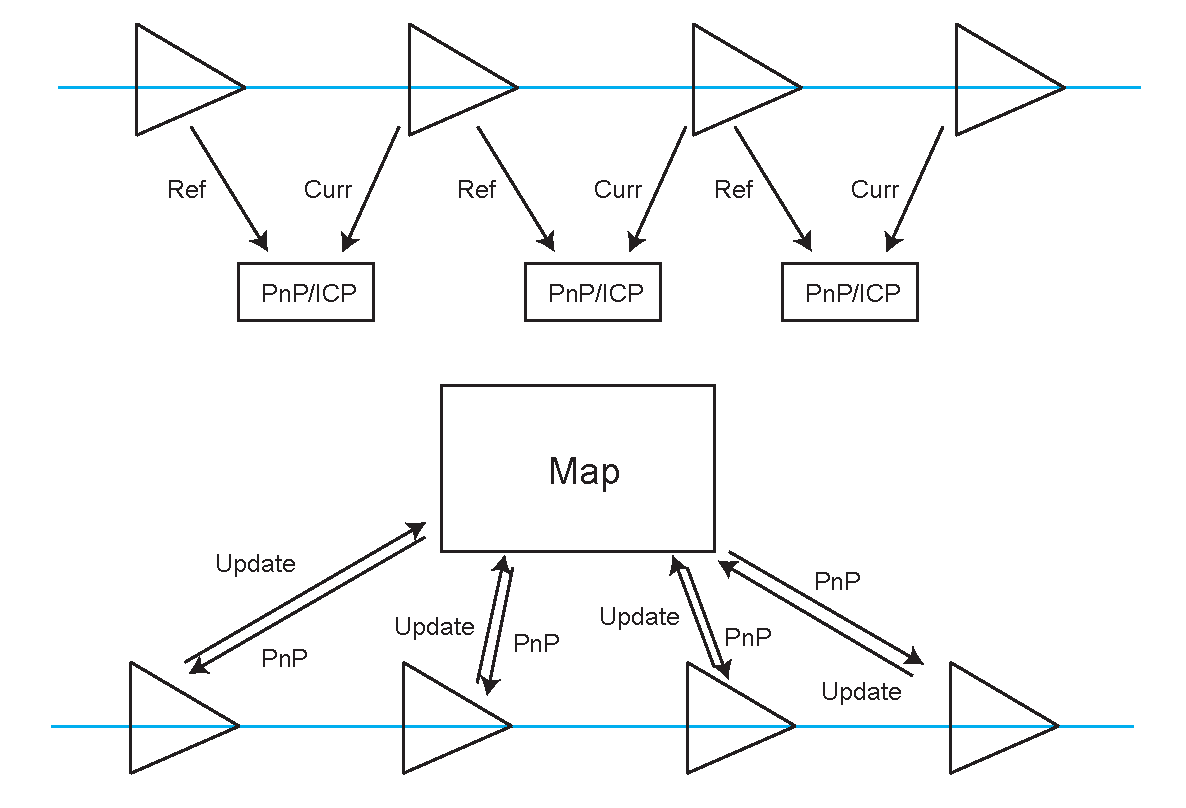
\includegraphics[width=0.9\linewidth]{designVO/vo04}\\
	\caption{两两帧VO与地图VO工作原理的差异。}
	\label{fig:vo04}
\end{figure}

在两两帧间比较时,我们只计算参考帧与当前帧之间的特征匹配和运动关系,在计算之后把当前帧设为新的参考帧。而在使用地图的VO中,每个帧为地图贡献一些信息,比如,添加新的特征点或更新旧特征点的位置估计。地图中的特征点位置往往是使用世界坐标的。因此,当前帧到来时,我们求它和地图之间的特征匹配与运动关系,即直接计算$\bm{T}_{\mathrm{cw}}$。

\newpage
这样做的好处是,我们能够维护一个不断更新的地图。只要地图是正确的,即使中间某帧出了差错,仍有希望求出之后那些帧的正确位置。请注意,我们现在还没有详细地讨论SLAM的\textbf{建图}问题,所以这里的地图仅是一个临时性的概念,指的是把各帧特征点缓存到一个地方构成的特征点的集合。

地图又可以分为\textbf{局部}(Local)地图和\textbf{全局}(Global)地图两种,由于用途不同,往往分开讨论。顾名思义,局部地图描述了附近的特征点信息——我们只保留离相机当前位置较近的特征点,而把远的或视野外的特征点丢掉。这些特征点是用来和当前帧匹配来求相机位置的,所以我们希望它能够做得比较快。另一方面,全局地图则记录了从SLAM运行以来的所有特征点。显然它的规模要大一些,主要用来表达整个环境,但是直接在全局地图上定位,对计算机的负担就太大了。它主要用于回环检测和地图表达。

在视觉里程计中,我们更关心可以直接用于定位的局部地图(如果决心要用地图的话)。所以本讲我们来维护一个局部地图。随着相机运动,我们往地图里添加新的特征点。我们仍然要提醒读者:是否使用地图取决于你对精度—效率这个矛盾的把握。我们完全可以出于效率的考量,使用两两无结构式的VO;也可以为了更好的精度,构建局部地图乃至考虑地图的优化。

局部地图的一件麻烦事是维护它的规模。为了保证实时性,我们需要保证地图规模不至于太大(否则匹配会消耗大量的时间)。此外,单个帧与地图的特征匹配存在着一些加速手段,但由于技术上比较复杂,我们的例程中就不给出了。

现在,来实现地图点类吧。我们稍加完善之前没有用到的MapPoint类,主要是它的构造函数和生成函数。

\begin{lstlisting}[language=c++,caption=slambook/project/0.4/include/myslam/mappoint.h]
class MapPoint
{
	public:
	typedef shared_ptr<MapPoint> Ptr;
	unsigned long      id_; // ID
	static unsigned long factory_id_; // factory id
	bool  good_; // whether a good point 
	Vector3d pos_; // Position in world
	Vector3d norm_; // Normal of viewing direction 
	Mat descriptor_; // Descriptor for matching 
	
	list<Frame*> observed_frames_;   // key-frames that can observe this point 
	
	int matched_times_; // being an inliner in pose estimation
	int visible_times_;  // being visible in current frame 
	
	MapPoint();
	MapPoint ( 
		unsigned long id, 
		const Vector3d& position, 
		const Vector3d& norm, 
		Frame* frame=nullptr, 
		const Mat& descriptor=Mat() 
	);
	
	inline cv::Point3f getPositionCV() const {
		return cv::Point3f( pos_(0,0), pos_(1,0), pos_(2,0) );
	}
	
	static MapPoint::Ptr createMapPoint();
	static MapPoint::Ptr createMapPoint ( 
		const Vector3d& pos_world, 
		const Vector3d& norm_,
		const Mat& descriptor,
		Frame* frame 
	);
};
\end{lstlisting}

主要的修改在VisualOdometry类上。由于工作流程的改变,我们修改了它的几个主要函数,例如,每次循环中要对地图进行增删、统计每个地图点被观测到的次数,等等\footnote{当然,从C++设计角度来说,保留之前的方式并使用继承会更有效地复用现有代码。}。这些事情是比较琐碎的,所以我们还是建议读者仔细看看GitHub上提供的源代码。重点观察以下几项:

\begin{enumerate}
	\item 在提取第一帧的特征点之后,将第一帧的所有特征点全部放入地图中:
\begin{lstlisting}[language=c++]
void VisualOdometry::addKeyFrame()
{
	if ( map_->keyframes_.empty() )
	{
		// first key-frame, add all 3d points into map
		for ( size_t i=0; i<keypoints_curr_.size(); i++ )
		{
			double d = curr_->findDepth ( keypoints_curr_[i] );
			if ( d < 0 ) 
				continue;
			Vector3d p_world = ref_->camera_->pixel2world (
				Vector2d ( keypoints_curr_[i].pt.x, keypoints_curr_[i].pt.y ), curr_->T_c_w_, d
			);
			Vector3d n = p_world - ref_->getCamCenter();
			n.normalize();
			MapPoint::Ptr map_point = MapPoint::createMapPoint(
				p_world, n, descriptors_curr_.row(i).clone(), curr_.get()
			);
			map_->insertMapPoint( map_point );
		}
	}
	map_->insertKeyFrame ( curr_ );
	ref_ = curr_;
}
\end{lstlisting}
	\item 后续的帧中,使用OptimizeMap函数对地图进行优化。包括删除不在视野内的点,在匹配数量减少时添加新点,等等。
\begin{lstlisting}[language=c++]
void VisualOdometry::optimizeMap()
{
	// remove the hardly seen and no visible points 
	for ( auto iter = map_->map_points_.begin(); iter != map_->map_points_.end(); )
	{
		if ( !curr_->isInFrame(iter->second->pos_) )
		{
			iter = map_->map_points_.erase(iter);
			continue;
		}
		float match_ratio = float(iter->second->matched_times_)/iter->second->visible_times_;
		if ( match_ratio < map_point_erase_ratio_ )
		{
			iter = map_->map_points_.erase(iter);
			continue;
		}
		double angle = getViewAngle( curr_, iter->second );
		if ( angle > M_PI/6. )
		{
			iter = map_->map_points_.erase(iter);
			continue;
		}
		if ( iter->second->good_ == false )
		{
			// TODO try triangulate this map point 
		}
		iter++;
	}
	
	if ( match_2dkp_index_.size()<100 )
		addMapPoints();
	if ( map_->map_points_.size() > 1000 )  
	{
		// TODO map is too large, remove some one 
		map_point_erase_ratio_ += 0.05;
	}
	else 
		map_point_erase_ratio_ = 0.1;
	cout<<"map points: "<<map_->map_points_.size()<<endl;
}
\end{lstlisting}
	我们刻意留空了一些地方,请感兴趣的读者自行完成。例如,你可以使用三角化来更新特征点的世界坐标,或者考虑更好地动态管理地图规模的策略。这些问题都是开放性的。

	\item 特征匹配代码。匹配之前,我们从地图中拿出一些候选点(出现在视野内的点),然后将它们与当前帧的特征描述子进行匹配。
\begin{lstlisting}[language=c++]
void VisualOdometry::featureMatching()
{
	boost::timer timer;
	vector<cv::DMatch> matches;
	// select the candidates in map 
	Mat desp_map;
	vector<MapPoint::Ptr> candidate;
	for ( auto& allpoints: map_->map_points_ )
	{
		MapPoint::Ptr& p = allpoints.second;
		// check if p in curr frame image 
		if ( curr_->isInFrame(p->pos_) )
		{
			// add to candidate 
			p->visible_times_++;
			candidate.push_back( p );
			desp_map.push_back( p->descriptor_ );
		}
	}
	
	matcher_flann_.match ( desp_map, descriptors_curr_, matches );
	// select the best matches
	float min_dis = std::min_element (
		matches.begin(), matches.end(),
		[] ( const cv::DMatch& m1, const cv::DMatch& m2 )
		{
			return m1.distance < m2.distance;
		} )->distance;
	
	match_3dpts_.clear();
	match_2dkp_index_.clear();
	for ( cv::DMatch& m : matches )
	{
		if ( m.distance < max<float> ( min_dis*match_ratio_, 30.0 ) )
		{
			match_3dpts_.push_back( candidate[m.queryIdx] );
			match_2dkp_index_.push_back( m.trainIdx );
		}
	}
	cout<<"good matches: "<<match_3dpts_.size() <<endl;
	cout<<"match cost time: "<<timer.elapsed() <<endl;
}
\end{lstlisting}

\end{enumerate}

除了现有的地图之外,我们还引入了“关键帧”(Key-frame)的概念。关键帧在许多视觉SLAM中都会用到,不过这个概念主要是给后端用的,所以我们在后面几讲再讨论对关键帧的详细处理。在实践中,我们肯定不希望对每个图像都做详细的优化和回环检测,那样毕竟太耗费资源。至少相机搁在原地不动时,我们不希望整个模型(地图也好、轨迹也好)变得越来越大。因此,后端优化的主要对象就是关键帧。

\clearpage
关键帧是相机运动过程当中某几个特殊的帧,这里“特殊”的意义是可以由我们自己指定的。常见的做法时,每当相机运动经过一定间隔,就取一个新的关键帧并保存起来\footnote{这在李代数上很容易实现,请想想怎么实现。}。这些关键帧的位姿将被仔细优化,而位于两个关键帧之间的那些东西,除了对地图贡献一些地图点外,就被理所当然地忽略掉了。

本节的实现也会提取一些关键帧,为后端的优化做一些数据上的准备。现在,读者可以编译这个工程,看看它的运行结果。本节的例程会把局部地图的点投影到图像平面并显示出来。如果位姿估计正确,它们看起来应该像是\textbf{固定在空间中一样}。反之,如果你感觉到某个特征点不自然地运动,那可能是相机位姿估计不够准确,或特征点的位置不够准确。

我们在0.4版没有提供对地图的优化,建议读者自行尝试一下。用到的原理主要是最小二乘和三角化,在前两讲已介绍过,不会太困难。

\begin{figure}[!htp]
\centering
\includegraphics[width=0.9\linewidth]{resources/designVO/vo04exp}
\caption{0.4版VO的运行截图,在两个不同时刻标记了路标投影点。}
\label{fig:vo04exp}
\end{figure}

\section{小结}

作为实践,本讲带领读者从零开始实现了一个简单的视觉里程计,为的是让读者对前面两讲介绍的算法有一个经验上的认识。如果没有本讲,你很难亲身体会到例如“特征点的VO大约能够实时处理多少个ORB特征点”这样的问题\footnote{当然这取决于你的机器的性能。}。我们看到,视觉里程计能够估算局部时间内的相机运动及特征点的位置,但是这种局部的方式有明显的缺点:

\begin{enumerate}
	\item 容易丢失。一旦丢失,我们要么“等待相机转回来”(保存参考帧并与新的帧比较),要么重置整个VO以跟踪新的图像数据。
	\item 轨迹漂移。主要原因是每次估计的误差会累积至下一次估计,导致长时间轨迹不准确。大一点的局部地图可以缓解这种现象,但它始终是存在的。
\end{enumerate}

值得一提的是,如果只关心短时间内的运动,或者VO的精度已经满足应用需求,那么有时候你可能需要的仅仅就是一个视觉里程计,而不用完全的SLAM。比如,某些无人机控制或AR游戏的应用中,用户并不需要一个全局一致的地图,那么轻便的VO可能是更好的选择。不过,本书的目标是介绍整个SLAM,所以我们还要走得更远一些,看看后端和回环检测是如何工作的。

\section*{习题}
\begin{enumerate}
	\item 本书使用的C++技巧你都看懂了吗?如果有不明白的地方,使用搜索引擎补习相关的知识,包括:基于范围的for循环、lambda表达式、智能指针、设计模式中的单例模式,等等。
	\item 在0.3版或0.4版的基础上,添加对地图进行优化的代码。或者,也可以根据PnP结果做一下三角化,消除RGB-D深度值的误差。
	\item 观察本讲代码是如何处理误匹配的。什么是RANSAC?阅读文献\cite{wiki:RANSAC}或搜索相关资料进行了解。
\end{enumerate}
